\chapter{Analyse et Conception de la plateforme Web}
 Nous présentons dans cette partie les phases d'analyse et de conception de
 l'application web. Il s'agira d'analyser le problème posé afin de concevoir une
 application répondant aux besoins qui ont été exprimés.

 \section{Analyse des besoins}

 Les besoins exprimés par la SGBF se résume en la mise en place d'un système
 permettant l'analyse vis à vis de la conformité d'un dossier de
 transfert déposé au guichet des opérations internationales. Partant de là, nous
 avons pu identifier les cas d'utilisations présentés dans le tableau
 \ref{tab:usecase}.

 Les principaux acteurs qui interagiront avec le système sont:
 \begin{description}
   \item[Le guichetier :] Il est chargé de la réception du dossier et de
     l'analyse de la cohérence et de la complétude du dossier. A la suite de
     cette analyse, il peut faire des observations sur le dossier.
   \item[L'administrateur :] Il a pour rôle la cration de nouveaux utilisateurs
     sur la plateforme. Il peut également consulter les statistiques.
 \end{description}
  \begin{table}
  \begin{center}
    \begin{scriptsize}
      \renewcommand{\arraystretch}{2}
      \begin{tabular}{|m{4cm}|m{10cm}|}
        \hline
        \rowcolor[gray]{.7}
        \bf \rule[-0.4cm]{0mm}{1cm} Cas d'utilisation &  \bf Description\\
        \hline
        Gérer un dossier & Enregistrer ou modifier un dossier. L'analyse
        conformité d'un dossier intervient juste après cette étape. \\ 
        \hline
        Faire des observations & Faire des observations sur la cohérence et la
        complétude du dossier \\
        \hline
        Gérer les accès au système & Création, modification et authentification
        des utilisateurs \\
        \hline
        Consulter des statistiques & Visualiser et exporter des données \\
        \hline
        Administrer le système & créer ou modifier les informations des
        utilisateurs. Attribuer des privilèges à un utilisateurs.\\
        \hline
      \end{tabular}
    \end{scriptsize}
    \caption{Les principaux cas d'utilisation du système \label{tab:usecase}}
  \end{center}
\end{table}

Le diagramme des cas d'utilisation résultant est le suivant. Il est présenté à
la figure \ref{fig:usecase}.

\begin{figure}[h!]
\begin{center}
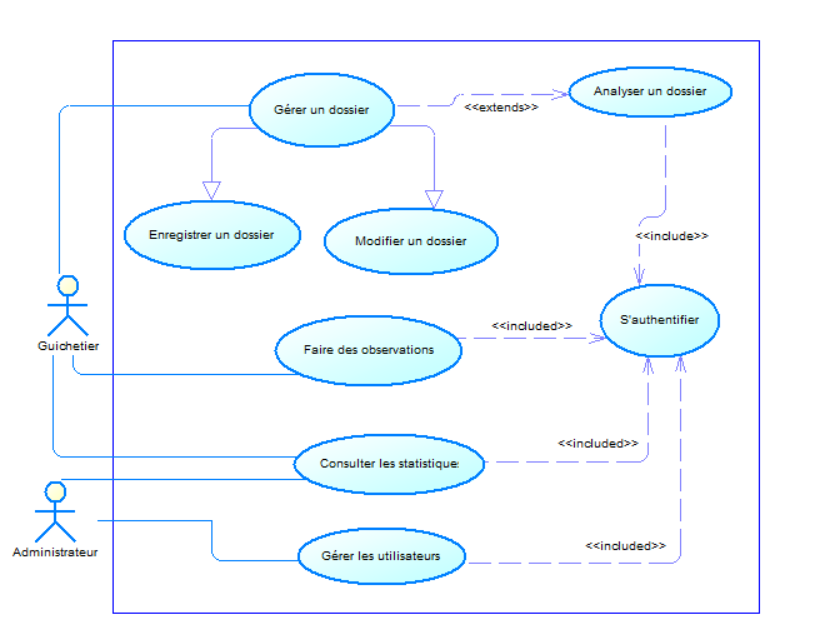
\includegraphics[width=14cm]
{images/usecase.PNG}
\caption{Diagramme des cas d'utilisation.\label{fig:usecase}}
\end{center}
\end{figure}
%


\begin{table}
  \begin{center}
    \begin{scriptsize}
      
      \begin{tabular}{|p{10cm}|}

        \hline
        Cas d'utilisation \og S'authentifier \fg\\
         \hline
         \uline{Titre: } S'authentifier \\
         \uline{Acteur Principal: } Guichetier \\
         \uline{Date de création :} 15/01/2020 \\
         \uline{Version: } 1.0 \\
         \uline{Auteur: } Ghislain Seghda\\
         \hline
         \textbf{Description des enchainements}\\
         \uline{Précondition}
         L'utlisateur dispose d'un ordinateur sur le réseau de la SGBF \\
         L'utilisateur dispose d'identifiant lui permettant d'accéder à la
         plateforme\\
         \hline
         \textbf{\uline{Scénario nominal}}\\
         \begin{enumerate}
           \item L'acteur se rend à l'adresse de l'application dans un
             navigateur depuis son ordinateur\\
           \item L'application se charge et présente la fenêtre
             d'authentification .\\
           \item L'acteur entre son nom d'utilisateur et son mot de passe puis
             valide ses entrées\[A1\], \[E1\]\\
           \item Le système vérifie l'authenticitédes informations et ouvre la
             page d'accueil.\\
         \end{enumerate}
         \textbf{\uline{Scénario alternatif}}\\
         \begin{enumerate}
           \item Le login et/ou le mot de passe sont incorrect pour la première
             ou la deuxième fois \\
           \item Le système informe l'acteur que les informations saisies sont
             incorrectes.\\
           \item Le scénario nominal reprend au point 1 \\
         \end{enumerate}
       \textbf{\uline{Scénario d'exception}}\\
       \begin{enumerate}
         \item L'acteur fourni pour la troisime fois des informations
           d'authentification erronées\\
         \item Le système bloque le compte de l'utilisateur\\
       \end{enumerate}
     \end{tabular}
   \end{scriptsize}
 \end{center}
\end{table}


\section{Conception}

Après l'identification des spécifications fonctionnelles du système, nous devons
procéder à sa conception. Pour y parvenir, nous avons suivi les étapes
suivantes:
\begin{itemize}
  \item Identification des entités ou concepts du domaine d'étude
  \item Identification et ajout des associations et des attributs
  \item Organisation et simplification du modèle en éliminant les classes
    redondantes
\end{itemize}
Le diagramme de classe obtenu est présenté à la figure \ref{fig:classe}.


\begin{figure}[h!]
\begin{center}
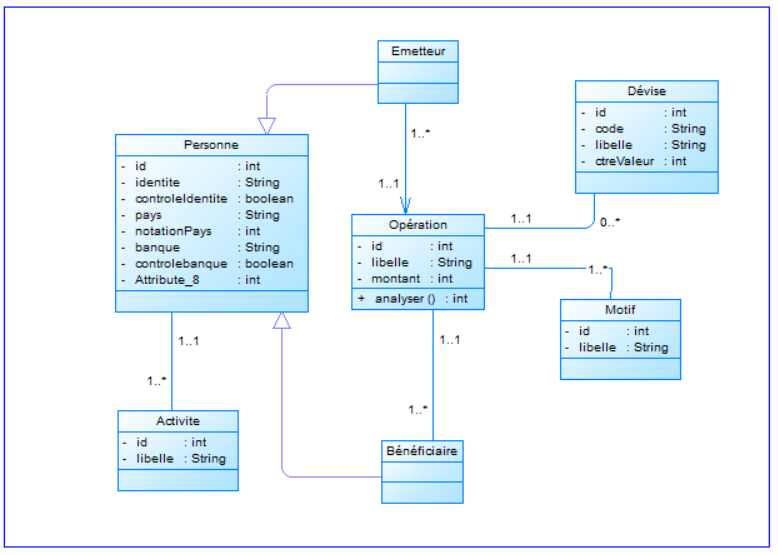
\includegraphics[width=14cm]
{images/classe.PNG}
\caption{Diagramme de classes.\label{fig:classe}}
\end{center}
\end{figure}

